% Standalone source of the figure fig:sphere of the continuum-limit paper.
% Build: pdflatex fig_sphere.tex (or lualatex); the paper includes the PDF.
% Grey scale only: tone, line style and marker shape carry the meaning.
\documentclass[border=2pt]{standalone}
% Shared preamble of the continuum-limit paper's standalone figures.
\usepackage{amsmath,amssymb,bm}
\usepackage{tikz}
\usetikzlibrary{calc}
\newcommand{\bS}{\mathbf{S}}
\newcommand{\bG}{\mathbf{G}}
\newcommand{\bK}{\mathbf{K}}
\newcommand{\bP}{\mathbf{P}}
\newcommand{\sinc}{\operatorname{sinc}}

\begin{document}
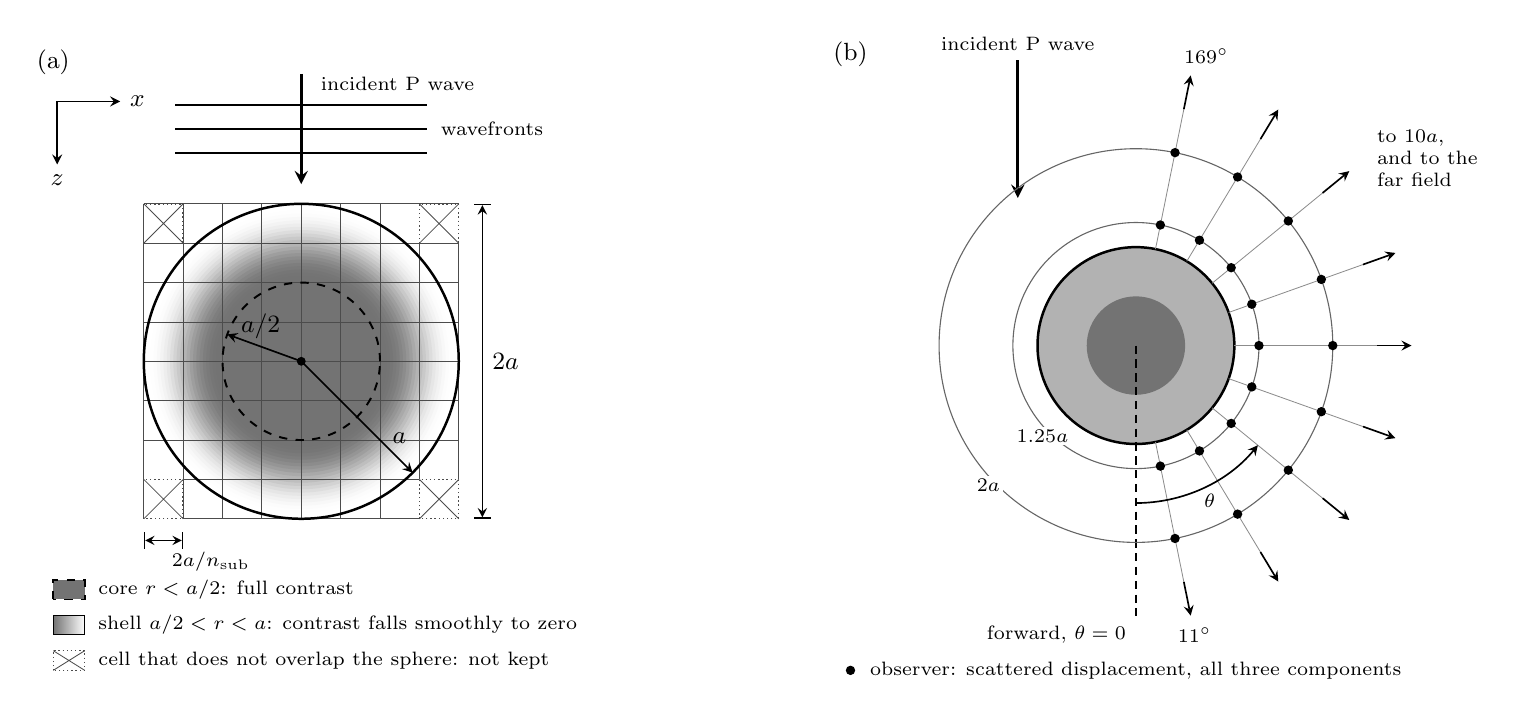
\begin{tikzpicture}[>=stealth, font=\small]
  % ---------------------------------------------------------------- (a) the body, the grid, the wave
  % section through the centre in the z-x plane; z points DOWN the page; unit = a/4 (one cell at n_sub = 8)
  \begin{scope}[x=0.5cm, y=0.5cm]
    \node at (-6.3,7.6) {(a)};
    % the graded shell: the smoothstep s = 10 x^3 - 15 x^4 + 6 x^5, x = (a - r)/(a/2), in 24 rings
    \foreach \i in {0,...,23} {
      \pgfmathsetmacro{\rr}{4 - \i*2/24}
      \pgfmathsetmacro{\xx}{(\i+0.5)/24}
      \pgfmathsetmacro{\tone}{55*(10*\xx^3 - 15*\xx^4 + 6*\xx^5)}
      \fill[black!\tone] (0,0) circle (\rr);
    }
    \fill[black!55] (0,0) circle (2);
    % the grid: the circumscribing cube cut into n_sub = 8 cells a side
    \foreach \k in {-4,...,4} {
      \draw[black!70, line width=0.3pt] (\k,-4) -- (\k,4);
      \draw[black!70, line width=0.3pt] (-4,\k) -- (4,\k);
    }
    % the four cells of this section that do not overlap the sphere: not kept
    \foreach \sx/\sy in {-4/-4, 3/-4, -4/3, 3/3} {
      \fill[white] (\sx,\sy) rectangle (\sx+1,\sy+1);
      \draw[black!70, densely dotted, line width=0.5pt] (\sx,\sy) rectangle (\sx+1,\sy+1);
      \draw[black!70, line width=0.3pt] (\sx,\sy) -- (\sx+1,\sy+1) (\sx,\sy+1) -- (\sx+1,\sy);
    }
    \draw[line width=0.9pt] (0,0) circle (4);
    \draw[dashed, line width=0.7pt] (0,0) circle (2);
    % radii
    \draw[->, line width=0.6pt] (0,0) -- (-45:4) node[pos=0.78, above right=-2pt] {$a$};
    \draw[->, line width=0.6pt] (0,0) -- (160:2) node[pos=0.55, above=-1pt] {$a/2$};
    \fill (0,0) circle (1.6pt);
    % the cell side
    \draw[|<->|, line width=0.5pt] (-4,-4.55) -- (-3,-4.55);
    \node[below, font=\scriptsize] at (-2.3,-4.6) {$2a/n_{\mathrm{sub}}$};
    \draw[|<->|, line width=0.5pt] (4.6,-4) -- (4.6,4) node[midway, right] {$2a$};
    % the incident P wave: plane wavefronts, travelling along +z (down), polarised along z
    \foreach \h in {5.3,5.9,6.5} \draw[line width=0.7pt] (-3.2,\h) -- (3.2,\h);
    \draw[->, line width=1.1pt] (0,7.3) -- (0,4.5);
    \node[right, align=left, font=\scriptsize] at (0.25,7.05) {incident P wave};
    \node[right, align=left, font=\scriptsize] at (3.3,5.9) {wavefronts};
    % axes
    \draw[->, line width=0.6pt] (-6.2,6.6) -- (-6.2,5.0) node[below] {$z$};
    \draw[->, line width=0.6pt] (-6.2,6.6) -- (-4.6,6.6) node[right] {$x$};
    % key
    \fill[black!55] (-6.3,-6.05) rectangle (-5.5,-5.55);
    \draw[dashed, line width=0.7pt] (-6.3,-6.05) rectangle (-5.5,-5.55);
    \node[right, font=\scriptsize] at (-5.4,-5.8) {core $r<a/2$: full contrast};
    \shade[left color=black!55, right color=white] (-6.3,-6.95) rectangle (-5.5,-6.45);
    \draw[line width=0.4pt] (-6.3,-6.95) rectangle (-5.5,-6.45);
    \node[right, font=\scriptsize] at (-5.4,-6.7) {shell $a/2<r<a$: contrast falls smoothly to zero};
    \draw[black!70, densely dotted, line width=0.5pt] (-6.3,-7.85) rectangle (-5.5,-7.35);
    \draw[black!70, line width=0.3pt] (-6.3,-7.85) -- (-5.5,-7.35) (-6.3,-7.35) -- (-5.5,-7.85);
    \node[right, font=\scriptsize] at (-5.4,-7.6) {cell that does not overlap the sphere: not kept};
  \end{scope}
  % ---------------------------------------------------------------- (b) the observers
  % same section; unit = a; scattering angle theta from the forward direction +z (down the page)
  \begin{scope}[shift={(10.6,0.2)}, x=1.25cm, y=1.25cm]
    \node at (-2.9,2.96) {(b)};
    \fill[black!30] (0,0) circle (1);
    \fill[black!55] (0,0) circle (0.5);
    \draw[line width=0.9pt] (0,0) circle (1);
    % the forward direction and the incident wave
    \draw[->, line width=1.1pt] (-1.2,2.9) -- (-1.2,1.5);
    \draw[densely dashed, line width=0.5pt] (0,0) -- (0,-2.75) node[anchor=north east, font=\scriptsize] {forward, $\theta=0$};
    \node[above, font=\scriptsize] at (-1.2,2.9) {incident P wave};
    % observer circles in the near field
    \draw[black!60, line width=0.4pt] (0,0) circle (1.25);
    \draw[black!60, line width=0.4pt] (0,0) circle (2);
    % nine scattering angles, equally spaced from 11.5 to 168.5 degrees
    \foreach \j in {0,...,8} {
      \pgfmathsetmacro{\th}{11.46 + \j*19.635}
      \draw[black!45, line width=0.3pt] ({1.0*sin(\th)},{-1.0*cos(\th)}) -- ({2.45*sin(\th)},{-2.45*cos(\th)});
      \fill ({1.25*sin(\th)},{-1.25*cos(\th)}) circle (1.7pt);
      \fill ({2*sin(\th)},{-2*cos(\th)}) circle (1.7pt);
      \draw[->, line width=0.6pt] ({2.45*sin(\th)},{-2.45*cos(\th)}) -- ({2.8*sin(\th)},{-2.8*cos(\th)});
    }
    % the angle
    \pgfmathsetmacro{\tha}{11.46 + 2*19.635}
    \draw[->, line width=0.6pt] (0,-1.6) arc (-90:{-90+\tha}:1.6);
    \node[font=\scriptsize, fill=white, inner sep=1pt] at ({1.75*sin(\tha/2)},{-1.75*cos(\tha/2)}) {$\theta$};
    % labels
    \node[font=\scriptsize, fill=white, inner sep=1pt] at (-0.95,-0.92) {$1.25a$};
    \node[font=\scriptsize, fill=white, inner sep=1pt] at (-1.5,-1.42) {$2a$};
    \node[right, align=left, font=\scriptsize] at (2.35,1.9) {to $10a$,\\and to the\\far field};
    \node[font=\scriptsize] at ({3.0*sin(11.46)},{-3.0*cos(11.46)}) {$11^\circ$};
    \node[font=\scriptsize] at ({3.0*sin(168.54)+0.12},{-3.0*cos(168.54)}) {$169^\circ$};
    \fill (-2.9,-3.3) circle (1.7pt);
    \node[right, font=\scriptsize] at (-2.8,-3.3) {observer: scattered displacement, all three components};
  \end{scope}
\end{tikzpicture}
\end{document}
